% ****** Start of file apssamp.tex ******
%
%   This file is part of the APS files in the REVTeX 4.1 distribution.
%   Version 4.1r of REVTeX, August 2010
%
%   Copyright (c) 2009, 2010 The American Physical Society.
%
%   See the REVTeX 4 README file for restrictions and more information.
%
% TeX'ing this file requires that you have AMS-LaTeX 2.0 installed
% as well as the rest of the prerequisites for REVTeX 4.1
%
% See the REVTeX 4 README file
% It also requires running BibTeX. The commands are as follows:
%
%  1)  latex apssamp.tex
%  2)  bibtex apssamp
%  3)  latex apssamp.tex
%  4)  latex apssamp.tex
%
\documentclass[%
 reprint,
%superscriptaddress,
%groupedaddress,
%unsortedaddress,
%runinaddress,
%frontmatterverbose, 
%preprint,
%showpacs,preprintnumbers,
%nofootinbib,
%nobibnotes,
%bibnotes,
 amsmath,amssymb,
 aps,
%pra,
%prb,
%rmp,
%prstab,
%prstper,
%floatfix,
10.5pt,
]{revtex4-1}

\usepackage{graphicx}% Include figure files
\usepackage{subfigure}
\usepackage{multirow}
\usepackage{array}
\usepackage{dcolumn}% Align table columns on decimal point
\usepackage{bm}% bold math
%\usepackage{hyperref}% add hypertext capabilities
%\usepackage[mathlines]{lineno}% Enable numbering of text and display math
%\linenumbers\relax % Commence numbering lines

%\usepackage[showframe,%Uncomment any one of the following lines to test 
%%scale=0.7, marginratio={1:1, 2:3}, ignoreall,% default settings
%%text={7in,10in},centering,
%%margin=1.5in,
%%total={6.5in,8.75in}, top=1.2in, left=0.9in, includefoot,
%%height=10in,a5paper,hmargin={3cm,0.8in},
%]{geometry}

\usepackage{xeCJK}
%\setCJKmainfont[ItalicFont={KaiTi}, BoldFont={KaiTi}]{KaiTi}
\usepackage{textcomp}
\usepackage{chemfig}
\usepackage[version=4]{mhchem}
\usepackage{fontspec}
\usepackage{listings}
\usepackage{xcolor}
\usepackage{xcolor} % 定制颜色
\definecolor{mygreen}{rgb}{0,0.6,0}
\definecolor{mygray}{rgb}{0.5,0.5,0.5}
\definecolor{mymauve}{rgb}{0.58,0,0.82}
\lstset{
backgroundcolor=\color{white},      % choose the background color
basicstyle=\footnotesize\ttfamily,  % size of fonts used for the code
columns=fullflexible,
tabsize=4,
breaklines=true,               % automatic line breaking only at whitespace
captionpos=b,                  % sets the caption-position to bottom
commentstyle=\color{mygreen},  % comment style
escapeinside={\%*}{*)},        % if you want to add LaTeX within your code
keywordstyle=\color{blue},     % keyword style
stringstyle=\color{mymauve}\ttfamily,  % string literal style
frame=single,
rulesepcolor=\color{red!20!green!20!blue!20},
% identifierstyle=\color{red},
language=Mathematica,
}

\usepackage[normalem]{ulem}

\newcommand{\chuhao}{\fontsize{42pt}{44.9pt}\selectfont}    % 初号, 1.5倍行距
\newcommand{\xiaochu}{\fontsize{30pt}{40pt}\selectfont}    % 小初, 1.5倍行距
\newcommand{\yihao}{\fontsize{26pt}{36pt}\selectfont}    % 一号, 1.4倍行距
\newcommand{\erhao}{\fontsize{22pt}{28pt}\selectfont}    % 二号, 1.25倍行距
\newcommand{\xiaoer}{\fontsize{18pt}{18pt}\selectfont}    % 小二, 单倍行距
\newcommand{\sanhao}{\fontsize{16pt}{24pt}\selectfont}    % 三号, 1.5倍行距
\newcommand{\xiaosan}{\fontsize{15pt}{22pt}\selectfont}    % 小三, 1.5倍行距
\newcommand{\sihao}{\fontsize{14pt}{21pt}\selectfont}    % 四号, 1.5倍行距
\newcommand{\sihaox}{\fontsize{14pt}{28pt}\selectfont}    % 四号, 1.5倍行距
\newcommand{\banxiaosi}{\fontsize{13pt}{19.5pt}\selectfont}    % 半小四, 1.5倍行距
\newcommand{\xiaosix}{\fontsize{12pt}{24pt}\selectfont} 	% 小四, 1.5倍行距
\newcommand{\xiaosi}{\fontsize{12pt}{18pt}\selectfont}     
\newcommand{\dawuhao}{\fontsize{11pt}{11pt}\selectfont}    % 大五号, 单倍行距
\newcommand{\wuhao}{\fontsize{10.5pt}{10.5pt}\selectfont}    % 五号, 单倍行距
\newcommand{\xiaowu}{\fontsize{9pt}{9pt}\selectfont}    % 五号, 单倍行距

%\usepackage[fntef]{ctexcap}
%\CTEXsetup[number={\chinese{section}、},format={\Large\bfseries}]{section}
%\setCJKfamilyfont{fangsong}{FangSong}                      %仿宋2312 fs  
%\newcommand{\fangsong}{\CJKfamily{fangsong}}  

\usepackage{wrapfig}
\usepackage{fancyhdr}
\usepackage{fancybox}   


\usepackage{tikz}
\usepackage{circuitikz}



\newcommand{\bra}[1]{\langle #1 |}
\newcommand{\ket}[1]{| #1 \rangle}
\newcommand{\bracket}[2]{\langle #1 | #2 \rangle}
\newcommand{\bracketl}[3]{\langle #1 | #2 | #3 \rangle}
\newcommand{\func}{\mathrm \,}
\newcommand{\define}[2]{
	\begin{definition}
	\begin{description}
	\item[#1]
	#2
	\end{description}
	\end{definition}
}

\newcommand{\sch}{Schr\"odinger}
\newcommand{\grad}{\nabla}
\newcommand{\ueq}{\neq}
\newcommand{\celsius}{\ensuremath{^\circ\hspace{-0.09em}\mathrm{C}}}
\newcommand{\unit}[2]{$#1 \, \mathrm{#2}$}

\begin{document}

%\preprint{APS/123-QED}

\title{Measurement of surface area of molecular sieves using BET theory}% Force line breaks with \\
%\thanks{A footnote to the article title}% give thanks

\author{Rui Li}
 %\altaffiliation[Also at ]{Physics Department, XYZ University.}%Lines break automatically or can be forced with \\
%\author{Second Author}%
%\email{3160102098@zju.edu.cn}
\affiliation{%
 Qiushi science class (chemistry)\\
 Chu Kochen Honor College
}%

%\collaboration{MUSO Collaboration}%\noaffiliation

\author{Zong Wei Huang}
% \homepage{http://www.Second.institution.edu/~Charlie.Author}
%\affiliation{
% Second institution and/or address\\
% This line break forced% with \\
%}%
\affiliation{
Qiushi science class (chemistry)\\
 Chu Kochen Honor College
}%
%\author{Delta Author}
%\affiliation{%
% Authors' institution and/or address\\
% This line break forced with \textbackslash\textbackslash
%}%

%\collaboration{CLEO Collaboration}%\noaffiliation

%\date{\today}% It is always \today, today,
             %  but any date may be explicitly specified

\begin{abstract}
The surface area of different models of molecular sieves are measured using BET theory adopting nitrogen as the adsorbates.
\begin{description}
\item[Keywords]
BET, molecular sieves
\end{description}
\end{abstract}

%\pacs{Valid PACS appear here}% PACS, the Physics and Astronomy
                             % Classification Scheme.
%\keywords{Suggested keywords}%Use showkeys class option if keyword
                              %display desired
\maketitle

\tableofcontents

\section{Introduction}

In 1916, Irving Langmuir first presented his model describing the absorption of species on a simple surface\cite{langmuir1918adsorption}. In 1938, Stephen Brunauer, P. H. Emmett and Edward Teller proposed the first theory of gases adsorption in multi-molecular layers, the BET theory, which has become a standard method to measure the surface area of the solid\cite{brunauer1938adsorption}. Its application includes analysis towards the physical structure of hardened cement paste, approximation of the surface area of activated carbon, and evaluation of catalysts.

\subsection{Langmuir: unimolecular equilibrium}
The surface adsorption can be regarded as a equilibrium
\begin{center}
\ce{A(g) + S <-> AS}
\end{center}
which represents the process of adduction between the two substances, \ce{A(g)}~being the gas molecule in the gas phase, while \ce{AS}~is the adduction product of the gas molecule and the molecule on the surface of the condensed substance.

\begin{figure}
\centering
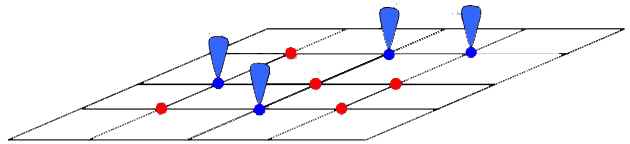
\includegraphics[width=0.45\textwidth]{figures/Langmuir_Adsorption_Model.jpg}
\caption{A simple graphic representation of the Langmuir adsorption model, where the red dots signify the unoccupied area, the blue points the occupied area.}
\end{figure}

Langmuir supposed that the adsorption rate is proportionl to the pressure of gas A and the area on the surface which haven't been occupied, while the desorption rate is proportional to the area occupied, which is shown by
\begin{equation}
k_{ad} p S_0 = k_{de} S_1
\end{equation}
where $k_{ad},k_{de}$ represent the reaction rate constant of the adsorption and the desorption respectively, $S_0,S_1$ the unoccupied and the occupied area, and $p$ the pressure of gas A in bulk phase.

Define the occupied percentage $\theta$
\begin{equation}
\theta = \frac{S_1}{[S]} = \frac{S_1}{S_0+S_1} = \frac{k_{ad}p}{k_{ad}p+k_{de}}
\end{equation}
and the adsorption equilibrium constant $K=\frac{k_{ad}}{k_{de}}$, then
\begin{equation}
\theta = \frac{Kp}{1+Kp}
\end{equation}


\subsection{BET: multi-molecular equilibrium}
\begin{figure}
\centering
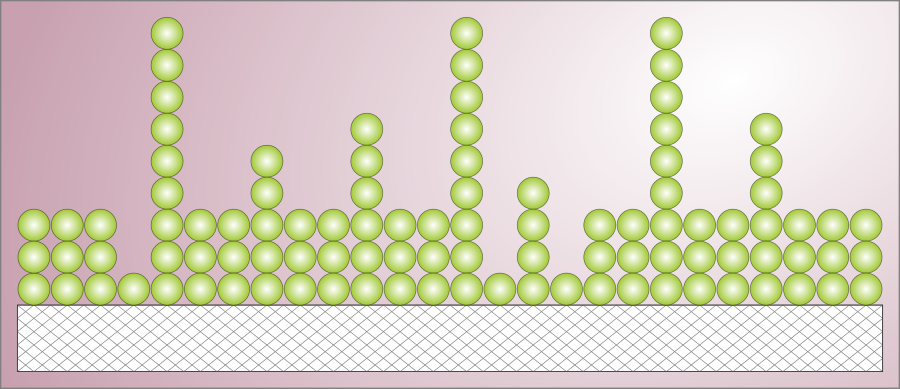
\includegraphics[width=0.45\textwidth]{figures/900px-BET_Multilayer_Adsorption.svg.png}
\caption{Sketch of the multilayered adsorption}
\end{figure}
It is supposed that many layers of adsorbed molecules can be formed on the surface of condensed substance, and $s_i$ is defined as the surface area that covered by $i$ layers of adsorbed molecules. When considering monolayer system, it is derived from the Langmuir's equation that
\begin{equation}
a_1 p s_0 = b_1 s_1 e^{-E_1/RT}
\label{firstlayer}
\end{equation}
where the term $e^{-E_1/RT}$ is separated from $K$ in the Langmuir's equation w.r.t. the Boltzmann distribution achieved between the adsorbed molecules and those in the bulk phase. For another system including only two layers of adsorbed molecules, the equilibrium is given by
\begin{equation}
a_2 p s_1 + b_1 s_1 e^{-E_1/RT} = b_2 s_2 e^{-E_2/RT} + a_1 p s_0
\end{equation}
with each term representing condensation on the first layer, evaporation from the first layer, evaporation from the second layer and condensation on the first layer, with $a_2,\, b_2,\, E_2$ similarly defined to $a_1,\, b_1$ and $E_1$. Considering that (\ref{firstlayer}) still holds in this system for the first layer, it is easily derived that
\begin{equation}
a_2 p s_1 = b_2 s_2 e^{-E_2/RT}
\end{equation}
Similar mechanism can be applied for an arbitrary index $i$, namely
\begin{equation}
a_i p s_{i-1} = b_i s_i e^{-E_i/RT}
\end{equation}
or
\begin{equation}
p s_{i-1} = g_i s_i e^{-E_i/RT}
\end{equation}
The total surface area is given by
\begin{equation}
A=\sum_{i=0}^{\infty} s_i
\end{equation}
and the total volume adsorbed is 
\begin{equation}
v = v_0 \sum_{i=0}^{\infty} i \cdot s_i
\end{equation}
where $v_0$ is the volume of gas adsorbed on unit area of the adsorbent surface when it is covered with a complete unimolecular layer of adsorbed gas. Then
\begin{equation}
\frac{v}{Av_0} = \frac{v}{v_0} = \frac{\sum_{i=0} i\cdot s_i}{\sum s_i}
\end{equation}
It is assumed that $E_i = E_j =E_L, g_i = g_j = g$ for $i,j \geq 2$, in the consideration of the similarity among these layers, and $s_i$ is given by
\begin{equation}
s_0 = c x^i s_0
\end{equation}
where $x = (p/g) e^{E/RT}, c = g g_1 e^{(E_1-E_L)/RT}$. Thus
\begin{equation}
\frac{v}{v_m} = \frac{c \sum_{i=1}^\infty i x^i}{1+ c \sum_{i=1}^\infty x^i}
\end{equation}
Then
\begin{equation}
\frac{v}{v_m} = \frac{cx}{(1-x)(1-x+cx)}
\label{BETmeta}
\end{equation}
w.r.t. the fact that
\begin{equation}
\sum_{i=1}^{\infty} x^i = \frac{x}{1-x} 
\end{equation}
(\ref{BETmeta}) indicates that endless adsorption will occur if $x \rightarrow 1$, which is evidently the result of $p \geqslant p_0$, $p_0$ representing the saturated vapor pressure of the adsorbed substance. Considering that $x \propto p$, it is assumed that
\begin{equation}
x= \frac{p}{p_0}
\end{equation}
Then (\ref{BETmeta}) is reduced to
\begin{equation}
\frac{v}{v_m} = \frac{c p}{(p_0-p)\left[1+(c-1)\frac{p}{p_0}\right]}
\end{equation}
or its linear form
\begin{equation}
\frac{c p}{V(p_0-p)} = \frac{1}{V_m}\left[1+(c-1)\frac{p}{p_0}\right]
\label{BETeq}
\end{equation}

\subsection{Methodology}
The use of nitrogen adsorption becomes one of the most widely-used method for the characterization of porous materials. The earliest reported studies of the adsorption nitrogen and other gases at liquid air temperature ($\sim$88 K) appear to have been made by Dewar and Ramsay in the course of their investigations of the composition of the atmosphere and the separation of the noble gases.\cite{SING20013}

Gas adsorption manometry is the method generally
used for the determination of adsorption
isotherms of nitrogen at the temperature of liquid
nitrogen ($\sim$77 K). This type of approach was
known as a `volumetric determination' (or alternatively
as the `BET volumetric method') since it
originally involved the measurement of gas volumes,
before and after adsorption. However, it
has been pointed out that it is no longer
appropriate to use the term `volumetric' since the
amount adsorbed is now generally evaluated by
measuring the change of gas pressure, rather than
a change in gas volume.

Two different operational procedures can be
used for the determination of the adsorption
isotherm. The conventional technique makes use
of a discontinuous, point-by-point procedure.
Successive amounts of the adsorptive are introduced
and at each stage the system is allowed
sufficient time to attain equilibrium, which of
course corresponds to a series of single points
on the adsorption isotherm. The continuous approach
is more recent and is dependent on the
principle of `quasi-equilibrium'. In this
case, the introduction of the adsorptive must be
slow enough to provide a continuous `equilibrium'
isotherm (i.e. with an infinite number of
points). If properly used, the continuous manometric
procedure has the great advantage that it
is possible to reveal inconspicuous features (e.g.
sub-steps), which may not be detectable by the
discontinuous method.

The aims of outgassing are two-fold —
(a) to reach a well-defined intermediate state by
the removal of physisorbed molecules; (b) to
avoid any drastic change as a result of ageing
or surface modification. Conventional vacuum
outgassing is the generally preferred technique,
but with fine powders, there is always a risk of
spurting. Spurting can be avoided and changes
in the adsorbent minimised by controlling the
rate of outgassing by the application of a form
of controlled rate thermal analysis, CRTA,
which is also termed `sample controlled thermal
analysis'.

\section{Results and Analysis}
degassed samples of 0.1215 g, 0.0910 g, 0.0814 g, 0.2577 g of 5A, TBX, 12X, 3A models of molecular sieves are weighed respectively and was subjected to adsorption analysis using Nova 4000e surface area analyzer, using nitrogen as the adsorbed substance and liquid nitrogen as the cooler. 

\begin{table}
\centering
\caption{$\frac{p/p_0}{V(1-p/p_0)} - p/p_0$ data of the four models of molecular sieves}
\begin{tabular}{c|cc}\hline
Model & $10^2 p/p_0 $ & $\frac{10^3 p/p_0}{V(1-p/p_0)/(\mathrm{g/cm^3})} $ \\ \hline
\multirow{6}{*}{5A} & 5.12330 & 0.399627 \\
& 9.83880 & 0.785563 \\
& 14.6168 & 1.21400 \\
& 19.5029 & 1.69589 \\
& 25.0192 & 2.30527 \\
& 29.8112 & 2.90425 \\\hline
\multirow{6}{*}{TDX} & 10.0683 & 0.397445 \\
& 12.8209 & 0.519410 \\
& 16.5952 & 0.699721 \\
& 20.8693 & 0.924308 \\
& 25.5477 & 1.19937 \\
& 30.1600 & 1.50676 \\\hline
\multirow{6}{*}{13X} & 5.08190 & 0.325157 \\
& 10.0178 & 0.657681 \\
& 14.9074 & 1.02933 \\
& 19.9015 & 1.45437 \\
& 25.0599 & 1.95200 \\
& 30.0583 & 2.50321 \\\hline
\multirow{6}{*}{3A} & 6.13740 & 4.21262 \\
& 10.1525 & 6.75755 \\
& 14.5214 & 9.56977 \\
& 20.0749 & 13.2330 \\
& 24.6837 & 16.3957 \\
& 29.8449 & 20.1105 \\\hline
\end{tabular}
\label{BETdata}
\end{table}

\begin{figure}
\centering
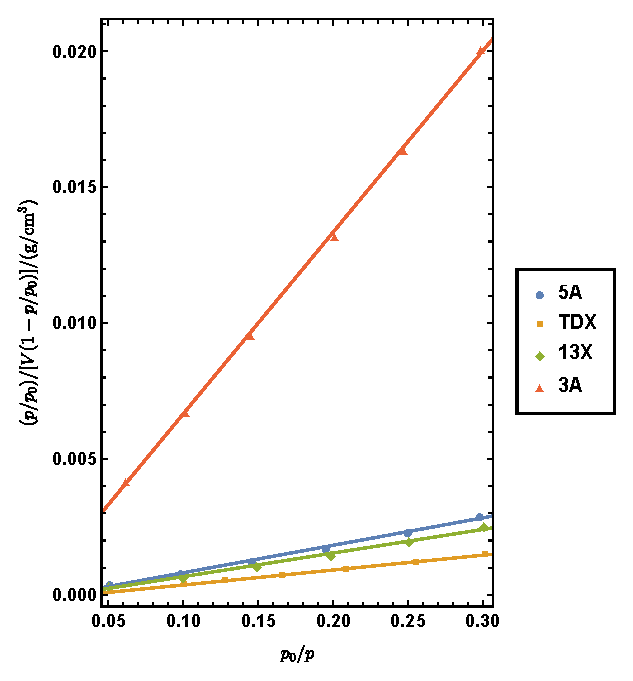
\includegraphics[width=0.45\textwidth]{figures/BETEX.eps}
\caption{$\frac{p/p_0}{V(1-p/p_0)} - p/p_0$ plot of the four models of molecular sieves}
\label{fg}
\end{figure}

The data obtained is shown in Table.\ref{BETdata}, with its graphic representation and analysis shown in Fig.\ref{fg}. The lines fitted are
\begin{align*}
&\frac{p/p_0}{V(1-p/p_0)}\bigg|_\text{5A} = 0.0101150  \frac{p}{p_0}-0.000201015 \\
&\frac{p/p_0}{V(1-p/p_0)}\bigg|_\text{TDX} = 0.00549478\frac{p}{p_0}-0.000188385 \\
&\frac{p/p_0}{V(1-p/p_0)}\bigg|_\text{13X} =  0.00869008 \frac{p}{p_0}-0.000200860 \\
&\frac{p/p_0}{V(1-p/p_0)}\bigg|_\text{3A} = 0.0668795\frac{p}{p_0}-0.0000369612 
   \end{align*}
with
\begin{align*}
& R^2 \bigg|_\text{5A} = 0.994307 \\
& R^2 \bigg|_\text{TDX} = 0.994965 \\
& R^2 \bigg|_\text{13X} = 0.992158 \\
& R^2 \bigg|_\text{3A} = 0.999460 
\end{align*}
Thus 
\begin{align*}
& V_m \bigg|_\text{5A} = 100.868 \,\mathrm{cm^3/g} \\
& V_m \bigg|_\text{TDX} = 188.452\,\mathrm{cm^3/g} \\
& V_m \bigg|_\text{13X} = 117.796 \,\mathrm{cm^3/g}\\
& V_m \bigg|_\text{3A} = 14.9605\,\mathrm{cm^3/g}
\end{align*}
and
\begin{align*}
& A \bigg|_\text{5A} = 439. \,\mathrm{m^2/g}\\
& A \bigg|_\text{TDX} = 821. \,\mathrm{m^2/g}\\
& A \bigg|_\text{13X} = 513. \,\mathrm{m^2/g}\\
& A \bigg|_\text{3A} = 65.2 \,\mathrm{m^2/g}
\end{align*}
w.r.t. the equation \ref{BETeq} and the fact that
\begin{equation}
A = V_m N_A \sigma_\text{\ce{N2}}, \quad \sigma_\text{\ce{N2}} = 16.2 \times 10^{-20} \, \mathrm{m^2}
\end{equation}
Deviation arises from the approximation of the BET theory, namely that the constant $g_i$ as well as $E_i$ is regarded the same among layers, which might lead to faulty description of the system, considering that a high pressure can be obtained on the adsorption surface due to the Lennard-Jone interactions among layers and between layers and the adsorbent surface\cite{shi2018high}. Deviation from adsorption equilibrium might also contribute to the error, whose clues can be found in the $R^2$ of the four samples, among which only 3A model cannot adsorb nitrogen into its pores, thus having least surface area measured, and the best linearity obtained. 

A closer look at the distribution of data points reveals a tendency of a positive second derivative of $\frac{p/p_0}{V(1-p/p_0)}$ towards $p/p_0$, which should be attributed to deviation from theoretical adsorption equilibrium, also indicating the problem of non-equal interaction among layers. Non-positive intercepts of the lines may also derive from these factors, which results in fluctuations of the linear fitting results.

\section{Conclusion}
The surface area of different models of molecular sieves are measured using BET theory adopting nitrogen as the adsorbates. The falty assumption of BET theory as well as deviation from adsorption equilibrium are considered to be the main error-contributing factors.
 




\bibliography{References}
\end{document}
